\documentclass[11pt,a4paper,final,notitlepage]{report}
\usepackage[utf8]{inputenc}
\usepackage{amsmath}
\usepackage{amsfonts}
\usepackage{amssymb}
\usepackage{fullpage}
\usepackage{graphicx}
\usepackage{url}
\renewcommand{\baselinestretch}{1.25} %Increase 

\makeatletter
\newcommand*{\toccontents}{\@starttoc{toc}}
\makeatother

\newcommand{\noNumberChapter}[2]{
    \setcounter{chapter}{#1}
    \setcounter{section}{0}
    \chapter*{#2}
    \addcontentsline{toc}{chapter}{#2}
}

\begin{document}

\title{Specialist Production Module\\
	   Renderman Ice Shader}

\author{Tom Minor - Level I\\
		Software Development for Animation, Games and Effects\\
		Bournemouth University - NCCA}

\maketitle

\renewcommand{\abstractname}{Project Overview}
\begin{abstract}
%% 			What's my focus area? (CG Ice Cubes)
\begin{center}
In this project I aimed to develop a \textit{physically based \textbf{Ice Cube Shader}} in \textit{Renderman Shading Language}.
\end{center}

\end{abstract}


\toccontents

%% Talk about :

%%			Why I chose shaders (wanted to learn them properly)
%%			Why I chose ice cube (wanted to do ice, but decided to pace myself and focus on just an ice cube, allowed me to collect primary research much easier than travelling to real life ice caves)
%%			Why Renderman (industry standard, fast, learning shaders once gives me a transferrable skill, offline rendering relieves me of the worry of having to make them behave well in real-time etc
\noNumberChapter{0}{Introduction}

\begin{center}
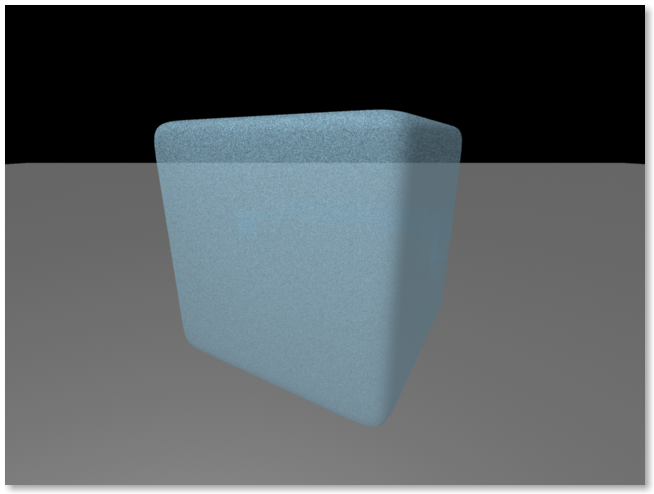
\includegraphics[scale=0.65]{../../../Pictures/testscene.png} 
\end{center}


Todo

\noNumberChapter{1}{Initial Research}
\section{Experiments with real ice cube and light}


\section{Related research from other papers}


\section{So what exactly is Renderman?}

%% Brief overview
%% Tutor suggested I look into superquads (insert picture)
%% Initially used Ian Stephenson's renderman compliant renderer, Angel
%% Due to noisy opacity and lack of shadows in quad shader, I moved onto prman
%%
%% Explain confusion between new RIS approach in PRMan compared to old REYES approach
%% RSL shaders can't be used with REYES, but RIS shaders are considerably more complex even if they are physically based

\section{Reading the documentation and tutorials}

Superquads \cite{superquad}

Pixar's Renderman documentation \cite{rmdocs} was invaluable for understanding the huge complexity of renderer in enough detail to begin writing useful shaders for it.

\noNumberChapter{2}{Production}
\section{Initial Tests}

%% Using superquads/angel

%% RSL

%% RIS Shaders?

\section{Results}
\section{Unforeseen Problems}

\noNumberChapter{3}{Conclusion}

\nocite{*}

\bibliographystyle{plain-annote}
\bibliography{bib_icereport}
\end{document}
